\chapter{Nucleon localization function}
\maketitle

\subsection*{\date{1 March 2017}}
Most recently I tried using Erik's modified version of HFBTHO to run for several constraints along $Q_{30}$ (or anywhere, really). What I'd like to do is use HFBTHO to generate densities quickly for $^{176}$Pt between $Q_{20}=241$ and $Q_{20}\approx 300$, and at $Q_{30}=4, 18$ (something I decided semi-arbitrarily once upon a time). I'm putting that on hold for a bit while I work on this inertia thing. Erik sent me some notes for perhaps getting the code to do what I want it to do, which are in my email. The files are currently in /p/lscratchh/matheson/locali-176Pt/hfbtho (/erik for testing his version of the code). Another thought I had was to try constraining $Q_{40}$ to something reasonable, and then releasing that constraint to find the actual density (hopefully) nearby.

\subsection*{17 May 2017}

Okay, I finally have some localizations worth talking about. I ended up settling on $^{176}$Pt, going along the axes $Q_{30}=6$ and $18$. Then once I got close to scission (and things started having trouble converging), I turned off the constraint on $Q_{30}$ thinking that would perhaps help with convergence and also round to fragments with the nearest whole number of particles. And it seems to have somewhat worked.

The more mass-asymmetric case ended up shifting from $Q_{30}=18$ to a little over 20, which is fine, though it should be noted that those calculations failed to converge and I'm not totally sure why. But taking them as fully-converged, correct solutions (in any case, I expect the densities to be pretty close to reality), we produce the fragments $^{93}$Nb, with an elongation $Q_{20}\approx3-5 b$, and $^{83}$Rb, with an elongation $Q_{20}\approx10-15 b$ (both fragments also show a small mass asymmetry of less than $1 b^\frac{3}{2}$, no doubt due to the heavy interactions between the two non-yet-fully-independent fragments). The weirdness of those two fragments leads me to wonder if perhaps I released the $Q_{30}$ constraint too late in the development of fragments, such that those fragments were determined (according to Nicolas's fission fragment toolkit in HFODD), \textit{at least} by $Q_{20}=285 b$, and probably well-before that.

In the more mass-symmetric case (but still with $Q_{30}\neq0$), it actually appears that the system chose to produce two equal-mass fragments ($^{88}$Y), and then to just deform one of them more than the other. So even though their mass and charge distribution is symmetric, the kinetic energy distribution is not.

Now, what I'm wondering is what is the benefit to all of this? I think the goal was that it would be nice to be able to identify fission fragments well before scission. Well, let's look at the output files I actually saved (why did I not think to save them all?! $\frown$). In the symmetric case, at $Q_{20}=285b$, the calculation actually failed to converge because the number of iterations was reached. But we did get an output, and according to that output the ``prefragments'' at that stage were $^{96}$Tc and $^{80}$Br. $Q_{20}=300b$ also failed to converge, and also gives two asymmetric fragments ($^{91}$Nb and $^{85}$Rb, but the localization plots \textit{look} symmetric, in case that means anything). When I got around to doing $Q_{20}=315b$, the fragments are actually \textit{still} not symmetric (according to the fragment toolbox) (I'll just print the output here):
\begin{verbatim}
*   -----------------------------------------------------------------------   *
*             |   LEFT  FRAGMENT (z < zN)   |   RIGHT FRAGMENT (z > zN)       *
*   -----------------------------------------------------------------------   *
*       <A>   |          88.9232            |          87.0768                *
*       <Z>   |          39.4393            |          38.5607                *
*       Etot  |         -33.0708            |         -46.1156                *
\end{verbatim}

\noindent And looking at the localization, you get the sense that it's going to be a \textit{fairly} even split, but you can't be totally sure because there are still some subtle differences between the two halves.

Okay, well, let's hold on here. Say we take these, and we have some sense of what the fragments are likely to be so we plot those as well. And then we sort of ``overlap'' the fragments and see if it matches up with the parent. So the way you could do this is to run calculations for several fragments in the region near where you expect fragments to appear, and give them the deformations you expect them to have at scission, and see if you can distinguish between the various fragments: do they have distinct clustering structure? Or perhaps some kind of unique shell-looking behavior?

\subsection*{18 May 2017}

Just by way of update on the mass-symmetric(-ish) case: I brought the quadrupole deformation out to 400 and still no signs of splitting. The properties of the fragments are equilibrating so perhaps it won't scission until it is able to conserve energy by doing so? Which would probably mean redistributing energy amongst the particles for a bit longer and then it'll be ready to break apart.

\subsection*{28 September 2017}

Apparently I never wrote about this before, but I wanted to test just \textit{how} distinct fragment shell structures were, and whether you'd be able to identify the fragments based on the localization. So I looked at a few possible fragmentations of $^{176}$Pt, just to see what we could learn. Here I'll show the proton localization plots for the lighter fragment as an example (the rest are stored on my computer somewhere). The fragments I chose to show (based on some semi-arbitrary fragment trajectory in the PES) were $^{82}$Se, $^{84}$Se, and $^{86}$Zr. $^{84}$Se has a magic number of neutrons (N=50); $^{82}$Se is two neutrons shy of a full shell; and $^{86}$Zr, with Z=40 and N=46, is not particularly close to a full shell in either nucleon.

\begin{figure}
  \begin{center}
    \subfigure[$^{86}$Zr]{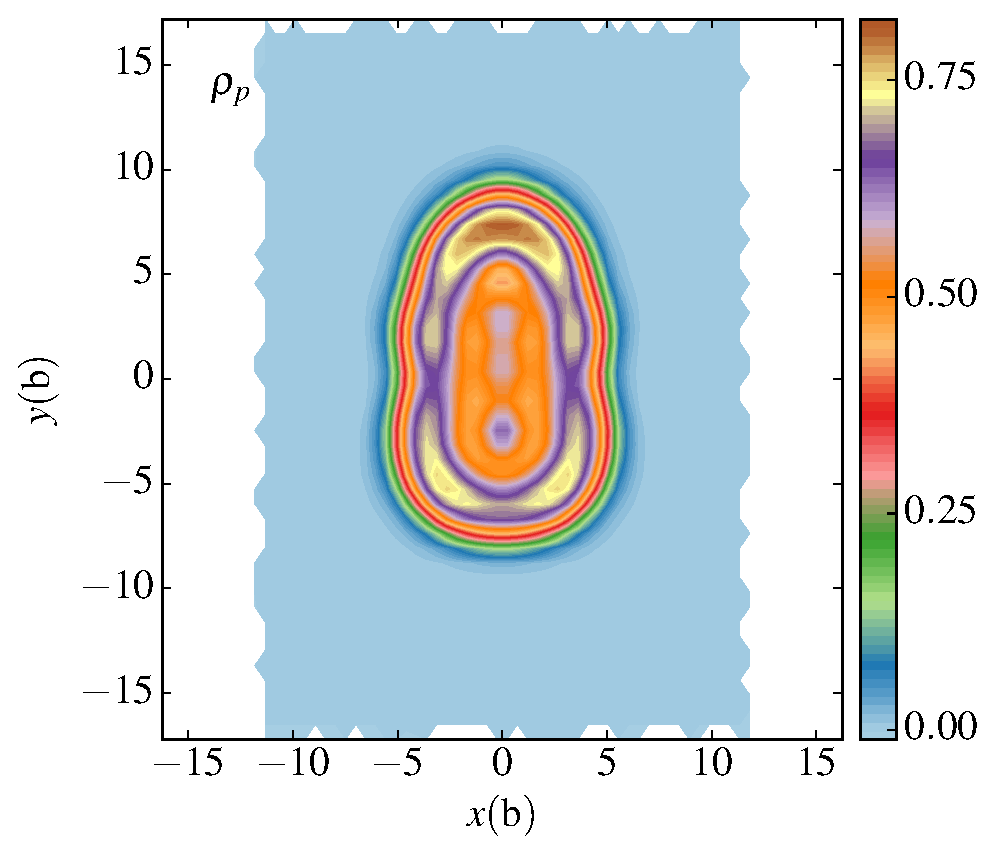
\includegraphics[width=0.3\linewidth]{86Zr-p-locali.eps}}\label{fig:86Zr-p-locali}
    \subfigure[$^{84}$Se]{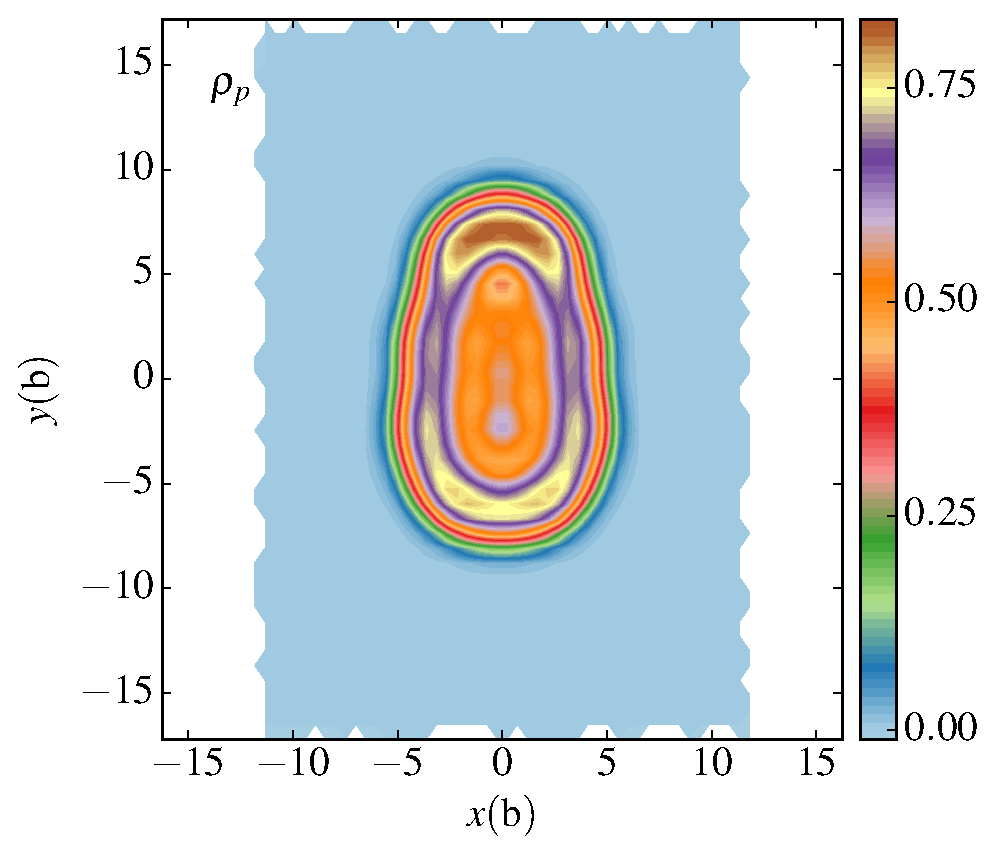
\includegraphics[width=0.3\linewidth]{84Se-p-locali.eps}}\label{fig:84Se-p-locali}
    \subfigure[$^{82}$Se]{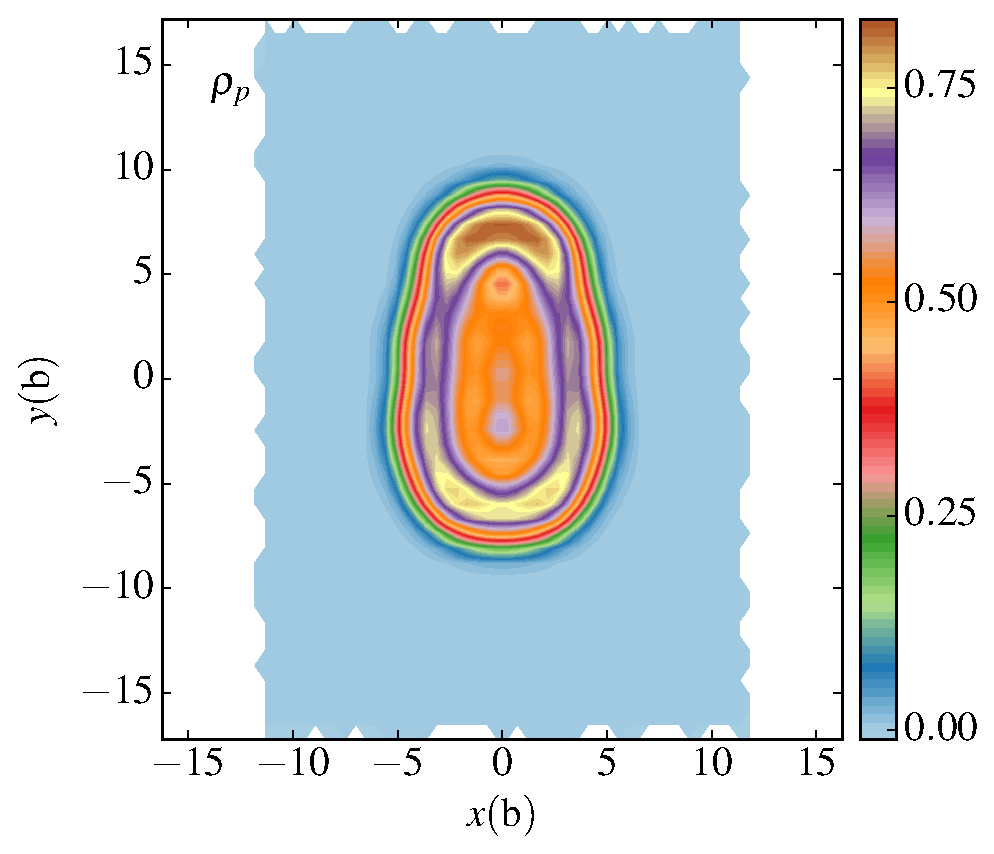
\includegraphics[width=0.3\linewidth]{82Se-p-locali.eps}}\label{fig:82Se-p-locali}
  \end{center}
  \caption{Proton spatial localization}
\end{figure}


As you can see, at this level, the selenium isotopes are virtually indistinguishable. Of course, that should not be surprising, as the number of protons stays the same. However, even looking at the neutron spatial localizations doesn't change the conclusion too much. The signatures are different but I don't know if they're so distinct that I'd be able to distinguish between them in a pre-scission developing fragment.

$^{86}Zr$ is distinct from the seleniums (as it should be, given that it differs by 6 protons). That said, I again don't know that I'd be able to pick them apart in a prefragment. Maybe.